\documentclass[10pt,twocolumn,letterpaper]{article}

\usepackage{cvpr}
\usepackage{times}
\usepackage{epsfig}
\usepackage{graphicx}
\usepackage{amsmath}
\usepackage{amssymb}
\usepackage{xcolor}
\usepackage{tabularx}
\usepackage{array}
\newcolumntype{C}[1]{>{\centering\arraybackslash}m{#1}}
\newcolumntype{R}[1]{>{\raggedleft\arraybackslash}m{#1}}
\newcolumntype{L}[1]{>{\raggedright\arraybackslash}m{#1}}
\usepackage{enumitem}
\usepackage{float}
\usepackage{pythonhighlight}
\definecolor{codegreen}{rgb}{0,0.6,0}
\definecolor{codegray}{rgb}{0.5,0.5,0.5}
\definecolor{codepurple}{rgb}{0.58,0,0.82}
\definecolor{backcolour}{rgb}{0.95,0.95,0.92}
\lstdefinestyle{mystyle}{
	backgroundcolor=\color{backcolour},   
	commentstyle=\color{codegreen},
	keywordstyle=\color{magenta},
	stringstyle=\color{codepurple},
	basicstyle=\ttfamily\footnotesize,
	breakatwhitespace=false,         
	breaklines=true,                 
	captionpos=b,                    
	keepspaces=true,                                                       
	showspaces=false,                
	showstringspaces=false,
	showtabs=false,                  
	tabsize=2,
	extendedchars=true, 
	literate={à}{{\'a}}1 {ù}{{\'u}}1 {è}{{\'e}}1 {é}{{\`e}}1 {ì}{{\'i}}1
}
\lstset{style=mystyle}
\usepackage{nicefrac}
% Include other packages here, before hyperref.

% If you comment hyperref and then uncomment it, you should delete
% egpaper.aux before re-running latex.  (Or just hit 'q' on the first latex
% run, let it finish, and you should be clear).
\usepackage[breaklinks=true,bookmarks=false]{hyperref}

\cvprfinalcopy % *** Uncomment this line for the final submission

\def\cvprPaperID{****} % *** Enter the CVPR Paper ID here
\def\httilde{\mbox{\tt\raisebox{-.5ex}{\symbol{126}}}}

% Pages are numbered in submission mode, and unnumbered in camera-ready
%\ifcvprfinal\pagestyle{empty}\fi
\setcounter{page}{1}
\begin{document}

%%%%%%%%% TITLE
\title{CNNs Ensemble for Facial Expression Recognition}

\author{
   Peagno Eleonora\\
   {\tt \small peagno.eleonora@studenti.unipd.it}
   %{\tt\small }
   % For a paper whose authors are all at the same institution,
   % omit the following lines up until the closing ``}''.
   % Additional authors and addresses can be added with ``\and'',
   % just like the second author.
   % To save space, use either the email address or home page, not both
   \and
   Peron Giovanni\\
   {\tt \small peron.giovanni@studenti.unipd.it}
   %{\tt\small secondauthor@i2.org}
   \and
   Rossi Daniel\\
   {\tt \small daniel.rossi@studenti.unipd.it}
   %{\tt\small secondauthor@i2.org}
}

\maketitle
%\thispagestyle{empty}

%%%%%%%%% ABSTRACT
\begin{abstract}
   %The ABSTRACT is to be in fully-justified italicized text, at the top
   %of the left-hand column, below the author and affiliation
   %information. Use the word ``Abstract'' as the title, in 12-point
   %Times, boldface type, centered relative to the column, initially
   %capitalized. The abstract is to be in 10-point, single-spaced type.
   %Leave two blank lines after the Abstract, then begin the main text.
   %Abstract should be no longer than 300 words.
   The facial expression recognition is a challenging task in machine learning field, and there is active research on this topic. Developing a machine able to understand human emotions is a fascinating goal. The purpose of this report is to exploit all the topics studied during the Vision and Cognitive Services course and others like Machine Learning and Deep Learning, in order to implement a system able to predict human emotions. We will describe how we realized this system specifying all the steps performed, from the first CNN to the final model we obtained. We will illustrate all the procedures we used for trying to achieve better results. Our target was not very high since this is a challenging task as we said, however with our final model we arrived to a prediction accuracy of \textbf{\textcolor{red}{71.52}}, that is better than human accuracy. Finally using this model we reached our goals implementing a nice application.
\end{abstract}

%%%%%%%%% BODY TEXT
\section{Introduction}
Facial expression recognition (FER) is an interesting and challenging problem in machine learning field. It is also a task that can be applied in many important applications. Facial expressions have an important role in every human interaction so developing a machine able to recognize and understand human expressions automatically can be very useful in many existing and novel fields \cite{2}. \\
One of these fields is behaviomedics, where systems are able to exploit automatically analysis of affective and social signals to aid diagnosis, monitoring and treating medical condition that alter behavior. Facial expression recognition can be also used in data analytics field, for example to understand emotions of people that are looking at ads or political debates and make statistics related to people's preferences. Another application field for facial expression recognition is human-computer interaction. Understanding human emotions would make the attitude of systems like vocal assistants or robots much closer to the way that humans interact with each other. Recognizing expressions could also be useful to improve the identification of micro facial expressions, which can be used in deceit detection applications. Due to all these possible applications, facial expressions recognition is widely studied also because recognizing human expressions in natural condition environment is a very challenging task. With this project we aim to build a facial expressions classifier able to reach and overtake human accuracy on this task. The main idea was to focus mostly on studying different types of models, in order to understand a good way to achieve valid outcomes. For this reason all preprocessing techniques that can be applied to the input data for improving classification results were not considered.
\begin{figure}[H]
   \centering
   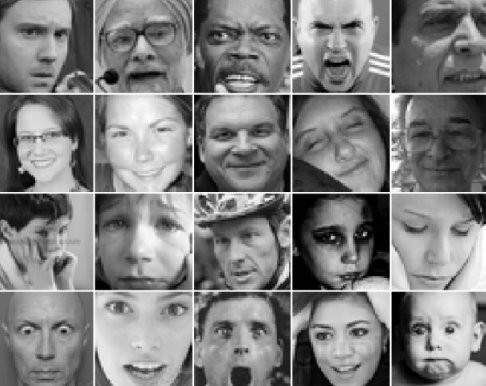
\includegraphics[width=0.8\linewidth]{./immagini/dataset.jpeg}
   \caption{Example of images from FER2013 dataset}
   \label{figure:imagesfer}
\end{figure}
The chosen dataset is the FER2013 it was selected after some researches, in figure \ref{figure:imagesfer} some examples of images of this dataset are reported. FER2013 was the desired dataset and the most suited for our purpose. Training a model with that dataset was the challenge with the right level of difficulty we was searching for. Moreover, FER2013 provides a very large set of examples well differentiated in terms of subjects age, face pose, illumination and other realistic conditions. Using the FER2013 data our goal was to realize an ensemble model compose by many types of Convolutional Neural Networks (CNNs), able to achieve a test accuracy greater than 65.5\%, that is the human accuracy measured on FER2013 dataset \cite{3}. Our target was reached using the final model described in the next sections \ref{subsection:ensemble}, which achieves test accuracy of 71.52\% on FER2013.

\section{Related Work}
The first step for reaching our goals has been a research of all the scientific papers related to the facial expression recognition. We found many different works related to the topic, all reviewed in \textit{``Deep Facial Expression Recognition: A Survey''} by S. Li and W. Deng \cite{paper}, thanks to this paper we could find a lot of correlated works about the same kind of classification we were looking for. We searched for all the works reported that were using the FER2013 dataset, trying to find a way to realize a model aligned with the best results achieved in the last years. We found six different papers related to the FER2013 dataset, they were classified by reached accuracy and type of neural networks used. After inspecting all these works we chose to follow the paper that achieved the best accuracy, moreover it was using an ensemble method and we were interested in understanding better this approach. So we decided to follow the methods used in \textit{``Facial Expression Recognition using Convolutional Neural Networks: State of the Art''} by C. Pramerdorfer and M. Kampel \cite{147}, that consists on an ensemble method made up by eight different CNNs of three different types, the accuracy reported for this method was 75.2\%. This paper has been enticing for us, because in it are explained the power and the bottlenecks of the CNNs models, moreover the final part of that paper was destined to explain how is possible to overcome the problems of CNNs. We found also other papers that we used as support to realize many different types of CNNs:
\begin{itemize}
   \item ``Very Deep Convolutional Networks
         for Large-Scale Image Recognition'' by K. Simonyan and A. Zisserman \cite{24};
   \item ``Going Deeper with Convolutions'' by C. Szegedy, W. Liu, Y. Jia, P. Sermanet, S. Reed, D. Anguelov, D. Erhan,
         V. Vanhoucke, and A. Rabinovich \cite{13};
   \item ``Deep Residual Learning for Image Recognition'' by K. He, X. Zhang, S. Ren, and J. Sun \cite{5}.
\end{itemize}
In the following table \ref{table:paperdiscarded} we report three of the works, executing facial expressions recognition task on the FER2013 dataset, we considered from \cite{paper}.

\begin{table}[h]
   \begin{center}
      \begin{tabular}{|C{2.2cm}|C{2.2cm}|C{1.6cm}|}
         \hline
         Papers                         & Network type          & Accuracy reached \\
         \hline\hline
         Zhang et al. \cite{Zhang}      & CNN Multitask Network & Test: 75.10      \\\hline
         Kim et al. \cite{Kim}          & CNN Network Ensemble  & Test: 73.73      \\\hline
         Pramerdorfer et al. \cite{147} & CNN Network Ensemble  & Test: 75.2       \\
         \hline
      \end{tabular}
   \end{center}
   \label{table:paperdiscarded}
\end{table}

\section{Dataset}
The FER2013 database was created by Pierre Luc Carrier and Aaron Courville. It was introduced during the ICML 2013 Challenges in Representation Learning and it is a large-scale and unconstrained database. This dataset was built collecting images in an automatic way using the Google image search API. In order to find useful faces images a research has been carried out combining a set of emotion related keywords with other words associated to gender, age or ethnicity. In this way about 600 strings were obtained and they were used to query the search API. Then all the images collected with this system have been cropped and resized to 48*48 pixels and they have been also converted to grayscale. We chose this dataset for many reasons, for example we found out that it is cited in many papers and we consider it well formed dataset for the reason that it contains images with different illumination, subjects with different age, pose and expression intensity, moreover some images have also occlusions. In general the images contained in the FER2013 dataset represent a good sampling under realistic conditions. The most important reason that pushed us to choose it is the huge number of images that it provides. Precisely it contains 28,709 training images, 3,589 validation images and 3,589 test images, so in total 35,887 images. For each image there is an associated class that represents seven different expression labels: Angry, Disgust, Fear, Happy, Sad, Surprised, Neutral. In \ref{figure:histogram1} we report an histogram showing the distribution of all the FER2013's labels.
\begin{figure}[H]
   \centering
   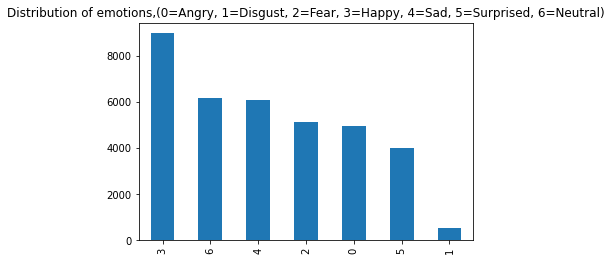
\includegraphics[width=1\linewidth]{./immagini/7_classi.png}
   \label{figure:histogram1}
\end{figure}
We tried to apply as few preprocessing techniques as possible, because we wanted to focus on the model performance providing to it a dataset not too optimized. We did this choice in order to emphasize the power of the model built, in the sense that we want a model able to reach interesting performance regardless of the goodness of the dataset provided to it. For this reasons we operated only some minimal preprocessing modification over the dataset, in order to prepare the data to be learned. First of all we noticed that the class disgust was not so big with respect to the others, so we decided to merge it with the angry class. Following a graph \ref{figure:histogram2}, is showing the distribution with merged classes.
\begin{figure}[H]
   \centering
   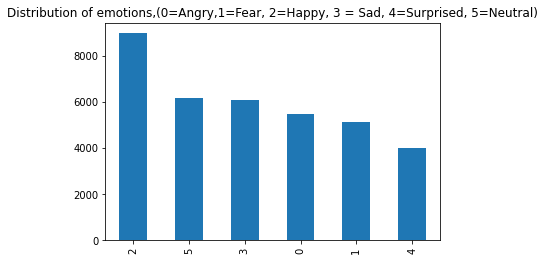
\includegraphics[width=1\linewidth]{./immagini/6_classi.png}
   \label{figure:histogram2}
\end{figure}
After this operation the classes were not so much leveled, in particular compared to happy class. In fact we had a lot of images for the happy class while the ones for the surprised emotion were very few. To solve this issue we decided to replicate the 60\% of the images of each class, excluding the happy class because as we said it already had enough images. In this way we made the images amount for each class more balanced and we reached the following distribution with a total amount of 52,025 images.
\begin{figure}[H]
   \centering
   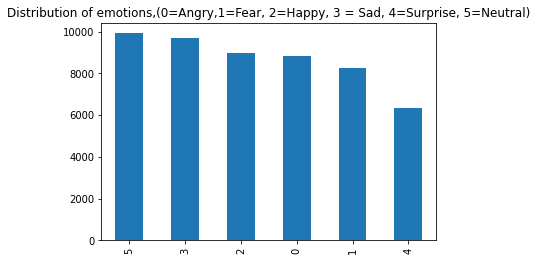
\includegraphics[width=1\linewidth]{./immagini/classi_bilanciate.png}
\end{figure}
Finally we performed a normalization operation over the dataset in order to provide to the model a numeric common scale. After all these needed preprocessing steps we obtained a training set formed by 44,847 images and a validation set and test set composed both by 3,589 images.\\
An evaluation of other dataset has been done, we considered also CK+ (CohnKanade) dataset that is also commonly used for evaluating FER systems. The first point that brought us to discard CK+ were the huge amount of data provided by FER2013, we decided that having as many images as possible was the right choice in order to develop a model that could well generalize, moreover the aim of reaching an interesting accuracy with FER2013 was more challenging. We decided to prefer FER2013 also because it appeared to us easier to work with, in fact FER2013 was provided in a csv file. A more important reason that led us to prefer FER2013 is the fact this one provides specified training, validation and test sets, instead CK+ does not, so in order to compare our results with other works it was the most appropriate dataset.

\section{Method}
The final model we built is an ensemble composed by different models from VGG, inception and ResNet types, we trained different models for each one of the type mentioned above in order to obtain predictions well generalized, the best models we developed is reported in table \ref{model:stable}.
\subsection{VGG}
\label{subsection:VGG}
For realizing this kind of network we followed the structure VGG-B descripted in \cite{24}. The VGG model is composed by several [CCPD] blocks and after flatting the data they are followed by some Fully connected (F) layers. We developed three different versions of this type of network, as shown below:
\\{\bf VGG\_v0} is composed by 4[CCPD], followed by 3F layers with respectively 25,25,6 neurons.
\\{\bf VGG\_v1} is composed by 4[CCBPD], followed by 4F layers with respectively 512,256,128,6 neurons.
\\{\bf VGG\_v2} is composed by 4[CBCBPD], followed by 4F layers with respectively 512,256,128,6 neurons.
VGG1 and VGG2 regularize the first C layer with L2 norm $\lambda=0.01$.
\subsection{Inception}
\label{subsection:Inception}
Inception model is a type of network developed from GoogLeNet \cite{13} with some modification according to the paper \cite{147}, we removed the initial pooling layer because the used FER2013's images were not so big. The network consist on several Inception (I) blocks, followed by a flatten and dropout layers and ending in a F layer with 6 neurons. For creating the I block we used a function that took a parameter $n$ representing the number of neurons of each block. We started with 64 neurons and we increment it of 32 after each I block. Every I block uses one C layer, padding same and L2 norm $\lambda=0.0002$, also we report kernel size (K) for the C layers. An I block is composed as follow:
\begin{enumerate}[noitemsep]%,topsep=0pt
   \item 1C relu, $\nicefrac{3}{4}\cdot n$, KernelSize (K) = (1,1)
   \item 2C relu, $\nicefrac{1}{2}\cdot n$, K=[(1,1),(3,3)]
   \item 2C relu, $\nicefrac{1}{8}\cdot n$, K=[(1,1), (5,5)]
   \item 1C relu, $\nicefrac{1}{4}\cdot n$, K=(5,5)
   \item PC relu, $\nicefrac{1}{4}\cdot n$, K=(1,1)
\end{enumerate}
All these blocks are concatenated in a [1C,2C,2C,PC] layer and after a P layer it becomes the input of next I blocks.
\begin{figure}[h]
   \centering
   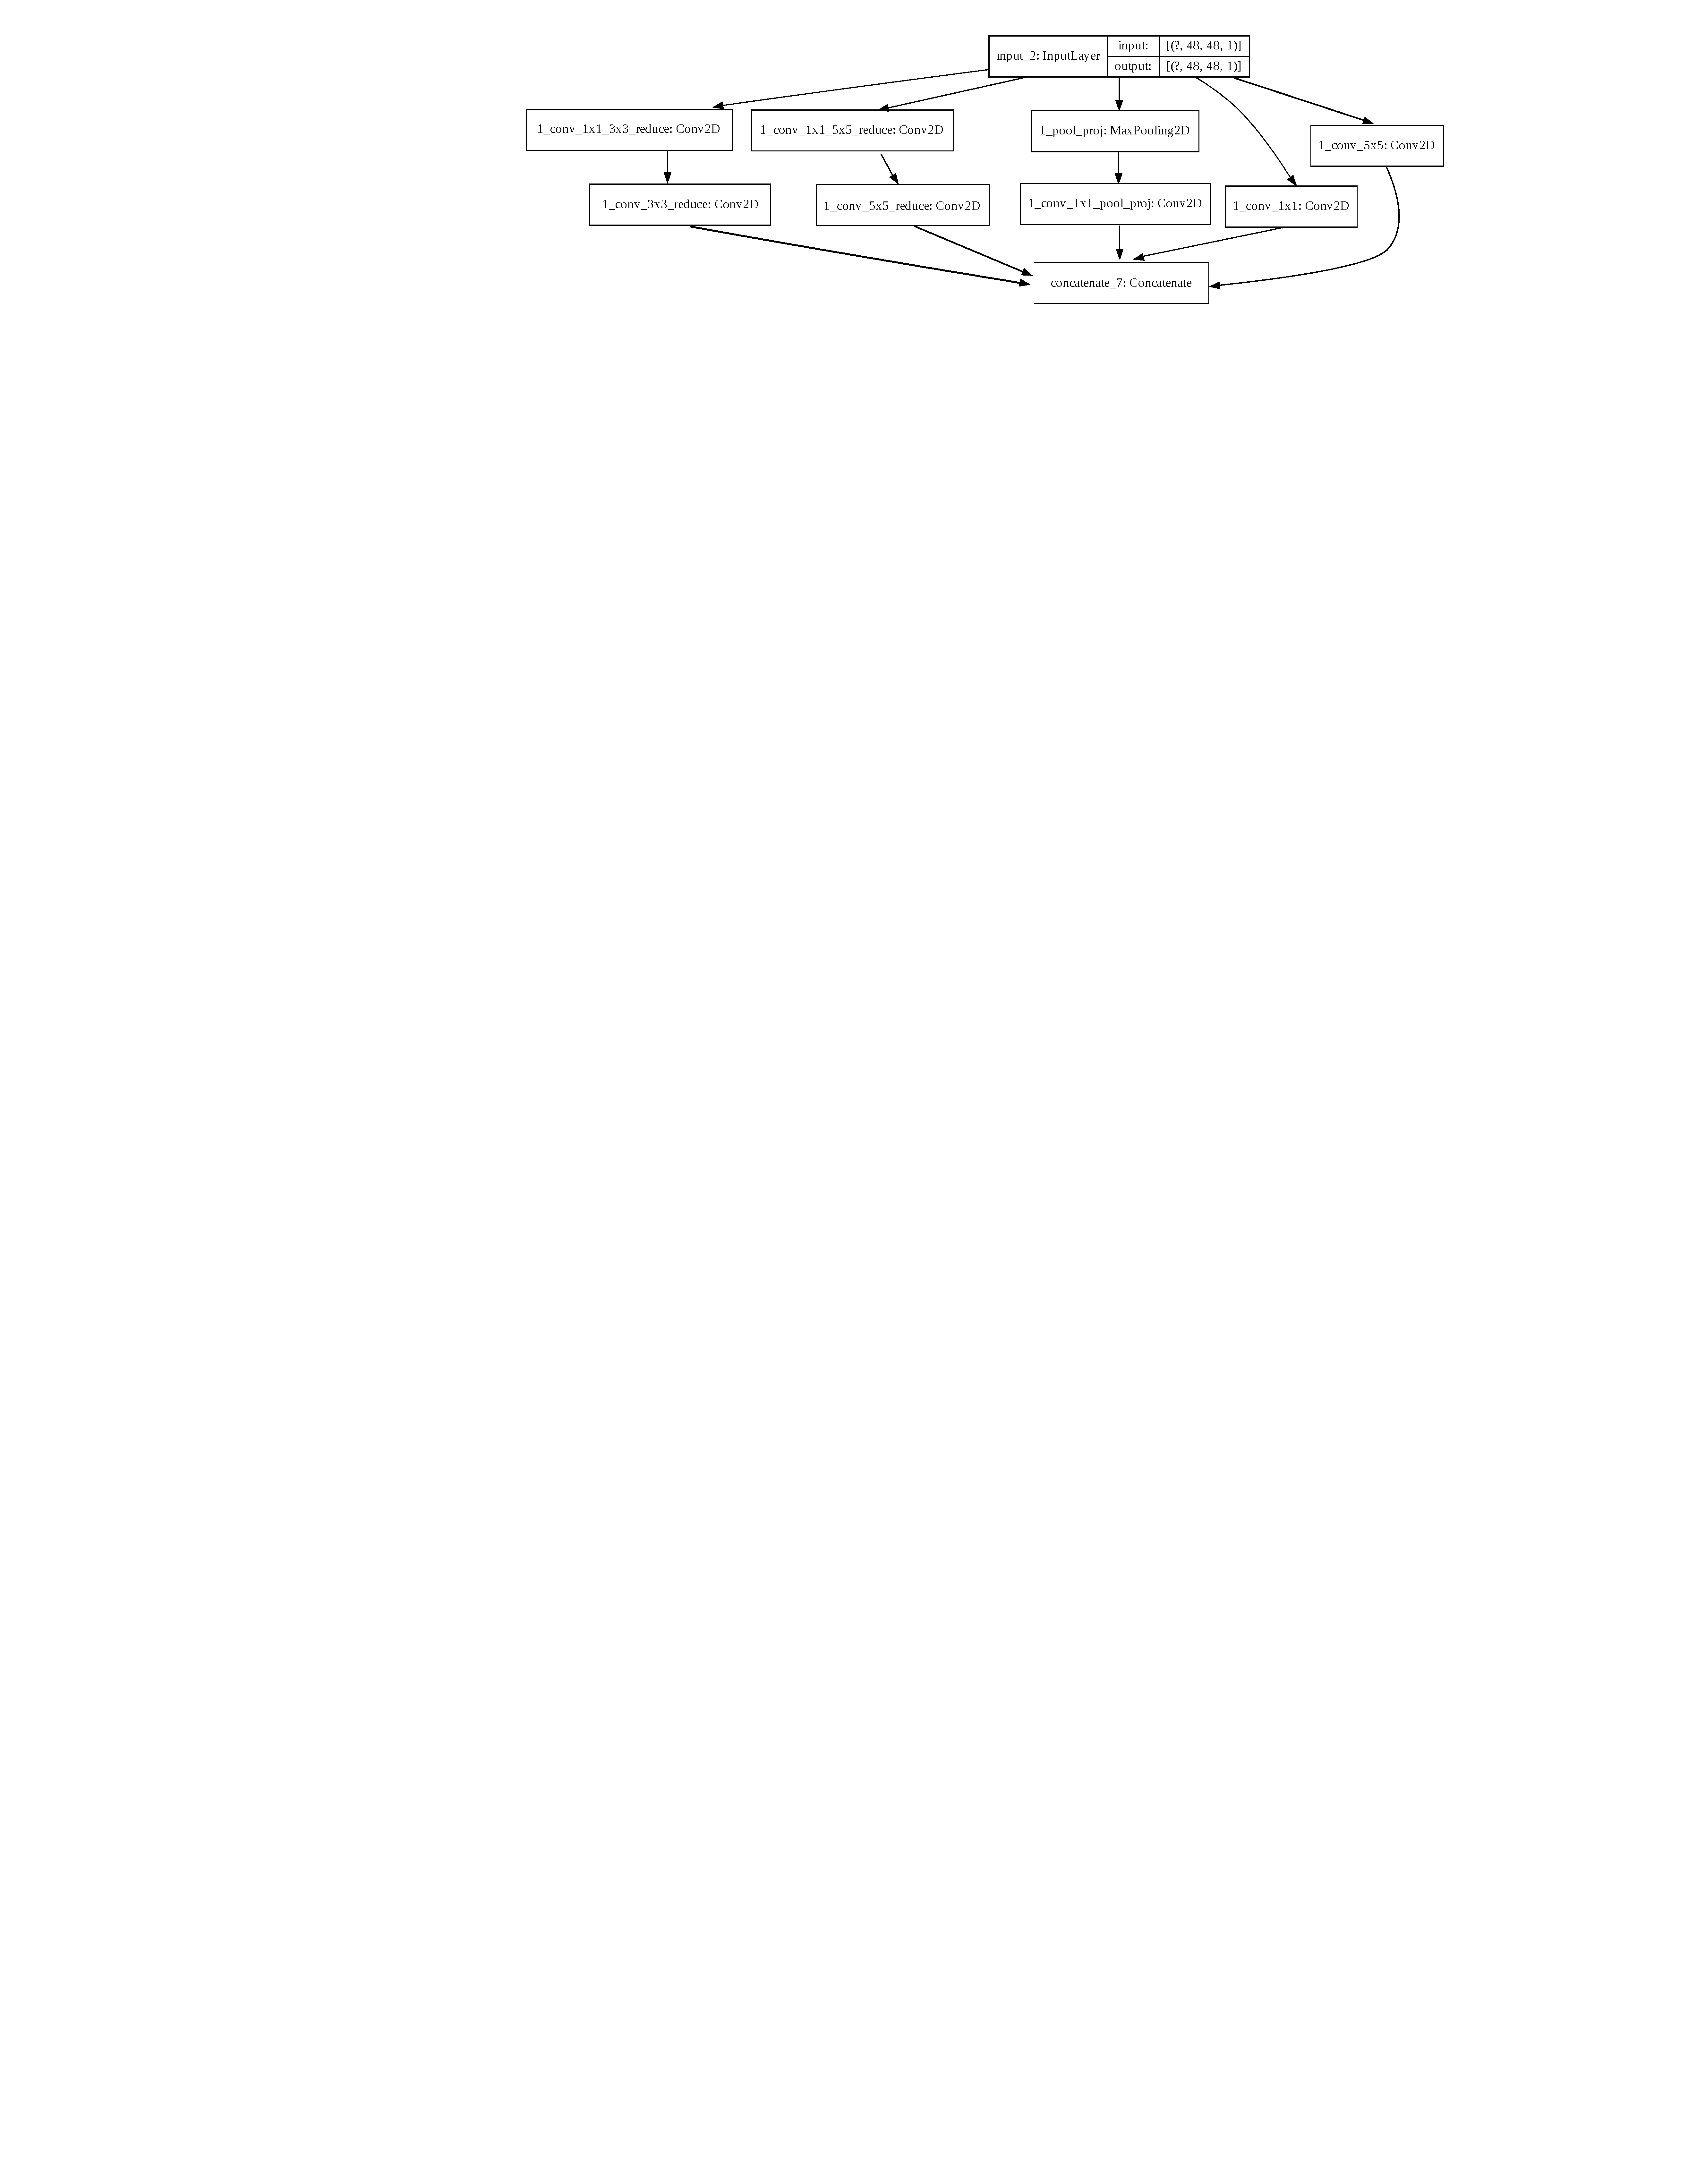
\includegraphics[width=0.9\linewidth]{./immagini/m_inception_v0.pdf}
   \caption{Representation of an I block}
\end{figure}
\vspace{-0.2cm}
\subsection{ResNet}
\label{subsection:ResNet}
ResNet model is a network that use Residuals (R) blocks. Each R consists on BatchNormalization (B) layer follow by [CFBC] layers with strides = 1, in the end there is an Add (A) layer, where we concatenate the output of [CFBC] and the initial B. Each C layer has kernel size = (3,3) and uses padding same, moreover the number of filter increase by a factor of 2 at each R block.
\begin{figure}[H]
   \centering
   \includegraphics[width=0.6\linewidth]{./immagini/residual_block.pdf}
   \caption{Representation of a residual block}
\end{figure}
At some fixed number of R blocks it is necessary to downsample the data and we substitute, into the A layer, the initial B with another C layer with strides = 2, also the first C layer of [CFBC] layers has stride = 2.
\begin{figure}[H]
   \centering
   \includegraphics[width=0.6\linewidth]{./immagini/residual_block_with_downsample.pdf}
   \caption{Representation of a residual block with downsample}
\end{figure}
\def\arraystretch{1.2}

\begin{table}[]

   \scriptsize
   %\begin{center}
   \begin{tabular}{L{0.8cm}C{0.6cm}C{3.4cm}C{0.6cm}C{0.8cm}}
      %\begin{tabular*}{5.5cm}{@{\extracolsep{\fill}}L{1.2cm}R{3cm}C{1.2cm}C{1.4cm}}
      \hline
      Name    & Type      & Architecture         & Depth & Params \\
      \hline\hline
      VGG0    & VGG\_v0   & 4[CCP] FF            & 10    & 4.8m   \\
      VGG1    & VGG\_v1   & 4[CCBP] FFF          & 11    & 5.9m   \\
      VGG2    & VGG\_v1   & 4[CCBP] FFF          & 11    & 5.9m   \\
      VGG3    & VGG\_v1   & 4[CCBP] FFF          & 11    & 5.9m   \\
      VGG4    & VGG\_v2   & CCBP 3[CBCBP] FFF    & 11    & 5.9m   \\
      Inc0    & Inception & CIPIIPIIPIIPF        & 16    & 4.8m   \\
      ResNet2 & ResNet    & C 2[R]5[R]5[R]2[R]PF & 30    & 15.6m  \\
      ResNet3 & ResNet    & C 3[R]4[R]6[R]3[R]PF & 34    & 21.3m  \\
      ResNet4 & ResNet    & C 3[R]4[R]6[R]3[R]PF & 34    & 21.3m  \\
      \hline
   \end{tabular}
   \label{model:stable}
   %\end{center}
   \caption{Summary of all the models realized. C, P, B, I, and F stands for convolutional, pooling, batch normalization, inception and fully connected layers respectively. 3[R] means group of three residual blocks. 4[CCP] means group of four CCP blocks. Final layer and dropout have been omitted.}

\end{table}

\subsection{Optimization}
In this part we explain how we trained the models and what tools we used in order to get the best model. Each model was trained with 150 epochs using Adam optimizer. Training this models were very long so we decided to use early stopping approach with a patience of 10 epochs and in some models we used a regularizer to help the loss function, when it was finding plateaus, by reducing the learning rate if there was no improvement on the validation loss function after 10 epochs.\\
We used checkpoints to save best weights during the training.\\
After the training phase we obtained about eleven models and we operated a selection over them, the latter will be explained in experiments section \ref{section:experiments}. We found out that the best combination of models consist on nine models, we have five VGGs, one Inception network and three ResNet models. 
%We combined them and we created two different ensemble, the first one was created using the arithmetic average and the second one instead uses the weighted average based on accuracy of the model on each class.


\subsection{Ensemble method}
\label{subsection:ensemble}
Our main goal was to train different models and then combine them in order to obtain a better generalization and improve the performance of the ensemble, the following figure \ref{figure:ensemblescheme} represents a scheme of the ensemble we tried:
\begin{figure}[H]
   \centering
   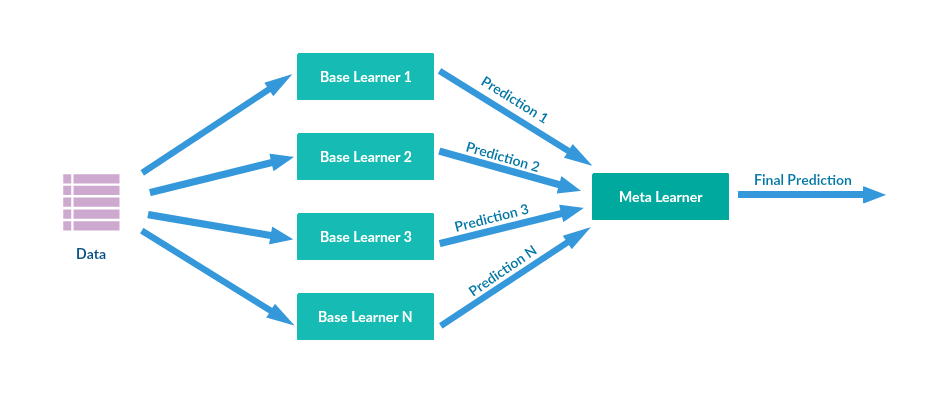
\includegraphics[width=1\linewidth]{./immagini/ensemble.png}
   \caption{Example of general ensemble method, in the meta-learner we compute the weighted average using the accuracy over the class and global accuracy for each model.}
   \label{figure:ensemblescheme}
\end{figure}
\def\arraystretch{1.2}
\begin{table}[H]
   %\begin{center}
   \scriptsize
   %\begin{tabular}{cccccccC{0.8cm}}
   \begin{tabular}{L{1.1cm}C{0.5cm}C{0.5cm}C{0.5cm}C{0.5cm}C{0.5cm}C{0.5cm}C{0.8cm}}
      \hline
      Name         & 0 (\%) & 1 (\%) & 2 (\%) & 3 (\%) & 4 (\%) & 5 (\%) & Test set (\%) \\
      \hline\hline
      ensemble9\_1 & 66.53  & 42.33  & 84.69  & 61.40  & 83.37  & 70.01  & 71.41         \\
      ensemble9\_2 & 66.53  & 42.13  & 84.69  & 61.56  & 83.37  & 70.51  & 71.41         \\
      ensemble9\_3 & 66.15  & 41.93  & 84.46  & 61.40  & 83.37  & 70.34  & 71.52         \\

      \hline
   \end{tabular}
   \caption{ 0=Angry,1=Fear,2=Happy,3=Sad,4=Surprised,5=Neutral, accuracies over the classes for each ensemble methods.}
   \label{table:accuracyensemble9}
   %\end{center}
\end{table}

\noindent\textbf{Ensemble9\_1}: we took the prediction from all models and then we calculated the simple average over the prediction of the same class, the best ensemble we obtained with this method had accuracy 71.41\% over the test set.\\
\textbf{Ensemble9\_2}: a natural step was to try weighted the average based on the accuracy of each model, but the final accuracy of the model was the same as the previous, the accuracy was 71.41\% over the test set.\\
\textbf{Ensemble9\_3}: we saw that some model in specific class were not so good, so we decided to weighted the average with class accuracy instead global accuracy of each model, the accuracy was 71.52\% over the test set. This is our final best ensemble model.
The following table \ref{table:modelli9}, illustrates all the models that compose the Ensemble9\_3.
\def\arraystretch{1.2}
\begin{table}[H]
   %\begin{center}
   \scriptsize
   %\begin{tabular}{cccccccC{0.8cm}}
   \begin{tabular}{L{1.1cm}C{0.5cm}C{0.5cm}C{0.5cm}C{0.5cm}C{0.5cm}C{0.5cm}C{0.8cm}}
      \hline
      Name    & 0 (\%) & 1 (\%) & 2 (\%) & 3 (\%) & 4 (\%) & 5 (\%) & Test set (\%) \\
      \hline\hline
      VGG0    & 53.53  & 49.19  & 76.87  & 51.60  & 81.92  & 57.00  & 63.58         \\
      VGG1    & 55.64  & 39.31  & 80.00  & 59.26  & 82.65  & 62.60  & 64.45         \\
      VGG2    & 60.80  & 31.85  & 80.33  & 61.86  & 76.86  & 61.12  & 65.78         \\
      VGG3    & 65.77  & 36.08  & 82.01  & 42.72  & 81.20  & 76.93  & 66.06         \\
      VGG4    & 60.03  & 40.72  & 81.56  & 47.93  & 79.03  & 72.98  & 67.18         \\
      Inc0    & 58.69  & 41.73  & 78.88  & 56.20  & 75.90  & 55.51  & 63.61         \\
      ResNet2 & 64.62  & 34.47  & 79.88  & 39.05  & 77.83  & 69.85  & 61.80         \\
      ResNet3 & 56.78  & 41.53  & 80.89  & 49.92  & 82.89  & 61.94  & 63.17         \\
      ResNet4 & 63.28  & 39.91  & 83.35  & 51.30  & 75.90  & 50.08  & 63.53         \\
      \hline
   \end{tabular}
   \caption{ 0=Angry,1=Fear,2=Happy,3=Sad,4=Surprised,5=Neutral, accuracy over the classes for each of the 9 models selected for the ensemble method.}
   \label{table:modelli9}
   %\end{center}
\end{table}

\section{Experiments}
\label{section:experiments}
In this section we will explain the process we made in order to realize the final ensemble model, illustrating all the steps we performed to build the needed networks and to improve the performance of them.
\subsection{Starting point}
Our experiments started from an unique convolutional neural network with a VGG like structure, which we called old\_net. This first network was trained with Adam optimizer and it reached a test accuracy of 60.27\%. We started from this first network and we searched for best methods in order to increase model's accuracy. Like we said in the previous sections \ref{subsection:ensemble}, the final model we obtained is an ensemble method composed by nine CNNs of three different types, that are VGG, Inception and ResNet. During the experiments process pursued in order to achieve models with best performance, we arrived to nine networks used for the final ensemble method discarding some networks from a set of eleven. 
In \ref{table:modelliscartati} we show two models we discarded.
\def\arraystretch{1.2}
\begin{table}[H]
   %\begin{center}
   \scriptsize
   %\begin{tabular}{cccccccC{0.8cm}}
   \begin{tabular}{L{1.1cm}C{0.5cm}C{0.5cm}C{0.5cm}C{0.5cm}C{0.5cm}C{0.5cm}C{0.8cm}}
      \hline
      Name     & 0 (\%) & 1 (\%) & 2 (\%) & 3 (\%) & 4 (\%) & 5 (\%) & Test set (\%) \\
      \hline\hline
      old\_net & 57.93  & 37.70  & 75.08  & 46.70  & 79.27  & 54.20  & 60.27         \\
      ResNet0  & 57.36  & 45.16  & 80.44  & 47.62  & 75.42  & 58.31  & 61.80         \\
      \hline
   \end{tabular}
   \caption{ 0=Angry,1=Fear,2=Happy,3=Sad,4=Surprised,5=Neutral, the models we rejected because got the ensemble worse.}
   \label{table:modelliscartati}
   %\end{center}
\end{table}
\subsection{Realizing three CNNs types}
After some modification tests, which did not lead so much improvement to our first network old\_net, we started following the model described in \cite{147}, implementing three CNNs architectures as described in \ref{subsection:VGG}, \ref{subsection:Inception}, \ref{subsection:ResNet}.\\
The initial modification has been the addition of B layers after every C layer. We also added some D layers, which have been useful to control the overfitting problem. Then we tried to use an SGD optimizer with initial learning rate = 0.1, L2 norm $\lambda=0.0001$, momentum = 0.9, batch size = 128. Initially we trained every network for 300 epochs, but then we decided to reduce the number of epochs to 150, for reasons of time needed for the training process. 

\subsection{Modifications for performance improving}
Following we describe all the modifications we made to each model we realized.
We added a learning rate regularizer in order to half the learning rate if the validation accuracy did not improve for 10 epochs, but with this optimizer we did not reach very interesting results due to the fact that sometimes the validation accuracy remained stuck on too low value, despite the learning rate regularizer. \\
For this reason we switched to use Adam optimizer, which being an adaptive learning method, solved our problem.
Using the tensorflow callback ReduceLROnPlateau\footnote{\url{https://www.tensorflow.org/api_docs/python/tf/keras/callbacks/ReduceLROnPlateau}} we added another system to control the learning rate. \\
With this method we help the loss function to get rid when the gradient descent is stuck in plateaus regions. What is done is reducing the learning rate parameter multiplying it for a defined factor if there is no improvement on the validation loss after a certain amount of epochs specified with the patience parameter. In order to save time and to optimize the accuracy of our models we decided to use the early stopping technique, trying different patience setting, in this way we were stopping the training when the model were not able to improve his validation loss for 10 epochs. We also use a checkpointer callback\footnote{\url{https://www.tensorflow.org/api_docs/python/tf/keras/callbacks/ModelCheckpointin}} in order to save the best model reached during the training process. In addition to the dropout we tried to use also an L2 regularizer in the VGG type networks. Combining all this settings we managed to get improved results.\\
Practically trying many different combination of modifications including the change of filters used in convolution layers and the addition of some more dense layer before the output layer. Like we reported on the table\ref{table:modelli9} we achieved a 67.18\% of test accuracy with a VGG neural network, that is our best result for a single network model. 

So, after many experiments we obtained eleven different models and we selected nine of them shown in table \ref{table:modelli9}. 

\subsection{Ensemble models}
Initially we used all the eleven models to build the ensemble model, like is illustrated in \ref{subsection:ensemble}\\
The ensemble model was built using a bagging technique, so retrieving the predictions made from all the single models and combining in a unique final prediction. 
\def\arraystretch{1.2}
\begin{table}[H]
   %\begin{center}
   \scriptsize
   %\begin{tabular}{cccccccC{0.8cm}}
   \begin{tabular}{L{1.1cm}C{0.5cm}C{0.5cm}C{0.5cm}C{0.5cm}C{0.5cm}C{0.5cm}C{0.8cm}}
      \hline
      Name          & 0 (\%) & 1 (\%) & 2 (\%) & 3 (\%) & 4 (\%) & 5 (\%) & Test set (\%) \\
      \hline\hline
      ensemble11\_1 & 66.73  & 43.34  & 84.58  & 59.72  & 82.40  & 70.51  & 70.95         \\
      ensemble11\_2 & 66.53  & 43.75  & 84.69  & 59.57  & 82.16  & 70.67  & 70.39         \\
      ensemble11\_3 & 66.92  & 43.75  & 84.35  & 60.03  & 82.40  & 71.33  & 70.95         \\
      \hline
   \end{tabular}
   \caption{ 0=Angry,1=Fear,2=Happy,3=Sad,4=Surprised,5=Neutral, in this ensemble we use all the 11 models developed.}
   \label{table:accuracymodelli}
   %\end{center}
\end{table}
\noindent\textbf{ensemble11\_1}: the predictions are combined making the average over all the predictions of the same class of each eleven models. In this way, that is putting together all the models we obtained a test accuracy of 70.95\%.\\
\textbf{ensemble11\_2}: at this point we tried to improve our performance weighting the results of each models based on accuracy of each model over the validation set, and we reach a test accuracy of 70.39\%, it is worst compared to the previous. \\
\textbf{ensemble11\_3}: we tried to weighting the predictions of each models with the accuracy over the classes for each model and we reach an accuracy of 70.95\%.\\
In order to compute this average we calculated a vector of weights to apply on the predictions of every model. To compute the weights we calculated the recall on the validation set for every prediction value returned by every model and we normalize it dividing by the sum of the weights computed.
The computation of the weights can be represented as follows
$\sum_{m=1,...,n} \frac{r_{m}}{\sum_{i=1,...,6} r_{m}[i]}$, where $r_m$ is a vector containing the recalls value for the model $m$
Having the weights normalized means that we have a level of the importance for every predicted class of every models.
The weighted average has been calculated as follows $\sum_{m=0,...,n} y_m\cdot w_m$, where in $y_m$ we have the predictions of the model $m$
and in $w_m$ we have the computed weights for the model $m$.

\subsection{Models selection}
After creating the first version of the ensemble we decided to try all different combination of the models from a minimum subset of six models to the maximum set of eleven models, we calculated for each combination the accuracy of the ensemble9\_3 of the selected models, we chose to use ensemble9\_3 because it seemed the better one. 
\\So the final model we obtained is the ensemble9\_3 model described in \ref{subsection:ensemble}, with which we obtain 71.52\% test accuracy.
\subsection{Application}
Finally we produced a python application for trying to use our model in order to predict emotions using the webcam of our personal computers.
We realized a simple application that retrieves images from webcam, it crops them and it converts them to grayscale in order to make a little bit similar to the FER2013 images.
The application starts the webcam and use our final model to predict an emotion and it shows the prediction below the webcam video that is being captured. In \ref{figure:ele1}, \ref{figure:ele2} we reported some application screenshot example.

\begin{figure}[H]
   \centering
   
\includegraphics[width=0.4\linewidth]{./immagini/ele_felice.png}
   \caption{Example of happyness prediction}
   \label{figure:ele1}
\end{figure}

\begin{figure}[H]
   \centering
   
\includegraphics[width=0.4\linewidth]{./immagini/ele_triste.png}
   \caption{Example of sadness prediction}
   \label{figure:ele2}
\end{figure}

% \begin{figure}[H]
%    \centering
%    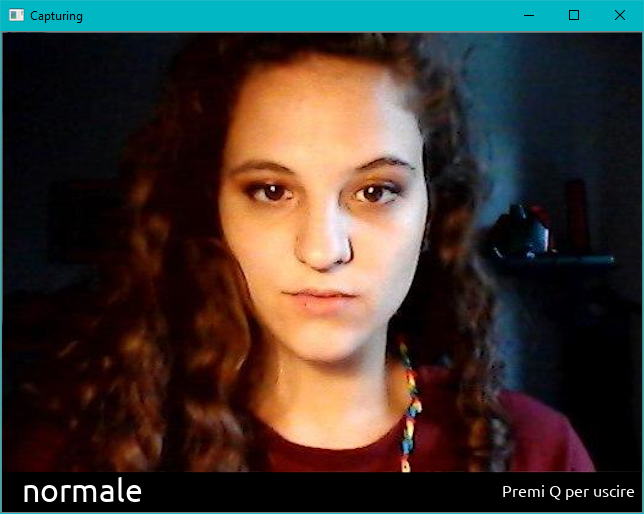
\includegraphics[width=0.8\linewidth]{./immagini/ele_neutrale.png}
%    \caption{Example of neutral prediction}
%    \label{figure:ele1}
% \end{figure}


\section{Conclusion}
We have achieved our aims which were to overtake the human accuracy estimated on the FER2013 dataset, which is 65.5\%. In fact our final model registers a test accuracy of 71.52\%, for this result we are satisfied.
Futhermore we overtake the accuracy reached from three papers, cited in \cite{paper}, in which were described models that perform the same task with the same dataset used by us, we are fullfilled for this result too. 
We can say it was very difficult to develop all the different models and it tooks a lot of times to train them, but we achieved a very good performance for each model. 
From this project we learnt how to make appropriate modification in the models, in order to obtain improvements of performance. We also understood how to produce an ensemble method with many networks and use it directly into an application. Surely we have explored only a part of the FER task, in fact the accuracy results obtained nowadays are greater than our. So there would be other techniques to apply in order to improve our model starting from data-augmentation to modifications of the ensemble model adding more types of CNNs and also improving the outcomes obtained from the ones we already use.
\newpage
{\small
   \bibliographystyle{ieee_fullname}
   \bibliography{egbib}
}

\end{document}
